%!TEX TS-program = pdflatex
%!TEX TS-options = -shell-escape
\RequirePackage{fix-cm}


\newcommand{\obenlinks}{Übungen zur Vorlesung Informatik I}   % hier Name der Veranstaltung eintragen
\documentclass[%
  paper=a4,
  fontsize=10pt,
  ngerman
  ]{scrartcl}

% Basics für Codierung und Sprache
% ===========================================================
  \usepackage{shellesc}                 % Compiler-Option -shell-escape benutzen!
  \usepackage[final]{graphicx}          % Einbindung von Grafiken
  \usepackage{subcaption}
%  \usepackage[utf8]{inputenc}          % Dateien sind UTF8-codiert
  \usepackage{babel}                    % deutsche Silbentrennung, etc.
  \usepackage[german=quotes]{csquotes}  % deutsche Anführungszeichen mit \enquote{...}
% ===========================================================

% Fonts und Typographie
% ===========================================================
  \usepackage[babel=true,final,tracking=smallcaps]{microtype}
  \DisableLigatures{encoding = T1, family = tt* }   % keine Ligaturen für Monospace-Fonts
% ===========================================================

% Farben
% ===========================================================
  \usepackage[usenames,x11names,final]{xcolor}
% ===========================================================

% Mathe-Pakete und -Einstellungen
% ===========================================================
  \usepackage{mathtools}               % Tools zum Setzen von Formeln
  \usepackage{amssymb}                 % übliche Mathe-Symbole
  \usepackage[bigdelims]{newtxmath}    % moderne Mathe-Font
  \allowdisplaybreaks                  % seitenübergreifende Rechnungen
  \usepackage{bm}                      % math bold font
  \usepackage{wasysym}                 % noch mehr Symbole
% ===========================================================

% TikZ
% ===========================================================
  \usepackage{tikz}
  \usetikzlibrary{arrows,arrows.meta}    % mehr Pfeile!
  \usetikzlibrary{calc}                  % TikZ kann rechnen
  \usetikzlibrary{positioning}
  \tikzset{>=Latex}                      % Standard-Pfeilspitze
% ===========================================================

% Seitenlayout, Kopf-/Fußzeile
% ===========================================================
  \usepackage{scrlayer-scrpage}
  \pagestyle{scrheadings}
  \usepackage[top=5cm, bottom=3cm, left=2.5cm, right=2cm]{geometry}
  \clearscrheadfoot 
  \setheadsepline{0.4pt}                            % Linie in Kopfzeile
  \setfootsepline{0.4pt}                            % Linie in Fußzeile
  \setkomafont{section}{\fontsize{14bp}{18.8bp}\normalfont}  % Schriftart der Section
  \setkomafont{subsection}{\fontsize{12bp}{16bp}\normalfont}                  
  \setkomafont{pagehead}{\textnormal}                 % Schriftart Kopfzeile
  \setkomafont{pagefoot}{\normalfont\footnotesize}  % Schriftart Fußzeile 
  \cfoot{\thepage}                                  % Seitenzahl unten Mitte
  \lohead{\obenlinks}                               % Titel oben links
  \raggedbottom                                     % Flattersatz
  \usepackage{setspace}                             % erweiterte Abstandsoptionen
  \onehalfspacing                                   % Zeilenabstand 1.5-fach
  \setlength{\parindent}{0pt}                       % Einrückung neuer Absätze
  \setlength{\parskip}{0.5\baselineskip}            % Abstand neuer Absätze
% ===========================================================

% Hyperref für Referenzen und Hyperlinks
% ===========================================================
  \usepackage[%
    hidelinks,
    pdfpagelabels,
    bookmarksopen=true,
    bookmarksnumbered=true,
    linkcolor=black,
    urlcolor=SkyBlue2,
    plainpages=false,
    pagebackref,
    citecolor=black,
    hypertexnames=true,
    pdfborderstyle={/S/U},
    linkbordercolor=SkyBlue2,
    colorlinks=false,
    backref=false]{hyperref}
  \hypersetup{final}
% ===========================================================

% Listen und Tabellen
% ===========================================================
  \usepackage{multicol}
  \usepackage[shortlabels]{enumitem}
  \setlist{itemsep=0pt}
  \setlist[enumerate]{font=\sffamily\bfseries}
  \setlist[itemize]{label=$\triangleright$}
  \usepackage{tabularx}
% ===========================================================

% minted
% ===========================================================
\usepackage{minted}
\setminted{%
  style=default,
  fontsize=\small,
  breaklines,
  breakanywhere=false,
  breakbytoken=false,
  breakbytokenanywhere=false,
  breakafter={.,},
  autogobble,
  numbersep=3mm,
  tabsize=4,
  linenos,
  frame=lines
}
\setmintedinline{%
  fontsize=\normalsize,
  numbers=none,
  numbersep=12pt,
  tabsize=4,
}

%%%%%%%%%%%%%%%%%%%%%%%%%%%%%%%%%%%%%%%%%%%%%%%%%%%%%%%%%%%
%%% Ab hier folgen nur noch vordefinierte Mathe-Befehle %%%
%%%%%%%%%%%%%%%%%%%%%%%%%%%%%%%%%%%%%%%%%%%%%%%%%%%%%%%%%%%

\newcommand{\BB}{\mathbb{B}}
\newcommand{\CC}{\mathbb{C}}
\newcommand{\NN}{\mathbb{N}}
\newcommand{\QQ}{\mathbb{Q}}
\newcommand{\RR}{\mathbb{R}}
\newcommand{\ZZ}{\mathbb{Z}}
\newcommand{\oh}{\mathcal{O}}            
\newcommand{\ol}[1]{\overline{#1}}
\newcommand{\wt}[1]{\widetilde{#1}}
\newcommand{\wh}[1]{\widehat{#1}}

\DeclareMathOperator{\id}{id}                        % Identität
\DeclareMathOperator{\pot}{\mathcal{P}}              % Potenzmenge

% Klammerungen und ähnliches
\DeclarePairedDelimiter{\absolut}{\lvert}{\rvert}    % Betrag
\DeclarePairedDelimiter{\ceiling}{\lceil}{\rceil}    % aufrunden
\DeclarePairedDelimiter{\Floor}{\lfloor}{\rfloor}    % aufrunden
\DeclarePairedDelimiter{\Norm}{\lVert}{\rVert}       % Norm
\DeclarePairedDelimiter{\sprod}{\langle}{\rangle}    % spitze Klammern
\DeclarePairedDelimiter{\enbrace}{(}{)}              % runde Klammern
\DeclarePairedDelimiter{\benbrace}{\lbrack}{\rbrack} % eckige Klammern
\DeclarePairedDelimiter{\penbrace}{\{}{\}}           % geschweifte Klammern
\newcommand{\Underbrace}[2]{{\underbrace{#1}_{#2}}}  % bessere Unterklammerungen
% Kurzschreibweisen für Faule und Code-Vervollständigung
\newcommand{\abs}[1]{\absolut*{#1}}
\newcommand{\ceil}[1]{\ceiling*{#1}}
\newcommand{\flo}[1]{\Floor*{#1}}
\newcommand{\no}[1]{\Norm*{#1}}
\newcommand{\sk}[1]{\sprod*{#1}}
\newcommand{\enb}[1]{\enbrace*{#1}}
\newcommand{\penb}[1]{\penbrace*{#1}}
\newcommand{\benb}[1]{\benbrace*{#1}}
\newcommand{\stack}[2]{\makebox[1cm][c]{$\stackrel{#1}{#2}$}}  % Präambel (ohne die geht nichts!)
\ihead{
  \section*{Informatik I - Gruppe 1 - Übungblatt 6}
  
  Ausgabe: 14.11.2022

  Abgabe: 21.11.1022

  Tutor: Tim Völker

  ~
}

\ohead{

  ~

  ~

  ~

  Ali Kurt 528961

  Thomas Kujawa 463620

  Felix Hoff 366927

  ~
}


\begin{document}
\graphicspath{ {./images/} }

\textbf{Aufgabe T6.1:} Rekursion (3 Punkte)

Gegeben sei eine Funktion $f$, definiert durch:

$$
f(n)= \begin{cases}2 \cdot f(n-1)+1 & \text { für } n \geq 1 \\ 1 & \text { sonst }\end{cases}
$$

(a) Geben Sie eine Wertetabelle an, die für $n=0,1,2,3,4,5,6$ das Ergebnis $f(n)$ angibt.

(b) Geben Sie den schrittweisen Ablauf der rekursiven Funktion als Expansion und Kontraktion für den Wert $n=4$ an.

(c) In welchem Verhältnis oder mathematischen Zusammenhang stehen $n \geq 0$ und der Funktionswert $f(n)$ ? Geben Sie die Funktion $f(n)$ in einer nicht-rekursiven Form an.

\newpage

\textbf{Aufgabe T6.2:} ADT Spezifikation (4 Punkte)

In der Vorlesung haben Sie abstrakte Datentypen (ADT) kennengelernt. Dabei wurde in der Vorlesung die Spezifikation eines Datentyps $A$ vorgestellt (Folie 291). Sie sollen nun 2 Realisierungen des Datentyps $A$ angeben, die nicht bereits in der Vorlesung vorgestellt wurden (Bool, Nat0 und anderen Datentypen aus Num) und welche die Signatur des Datentyps $A$ realisieren. Überprüfen Sie für beide Realisierungen, ob diese die Spezifikation erfüllen.

\newpage

\textbf{Aufgabe P6.3:} Binomialkoeffizienten / Pascalsches Dreieck (2 Punkte)

Zur Ermittlung der Binomialkoeffizienten $\left(\begin{array}{l}n \\ k\end{array}\right)$ kann das Pascalsche Dreieck zu Hilfe gezogen werden. Den passenden Koeffizienten findet man in der $n$-ten Zeile an der $k$-ten Stelle:

$\begin{array}{cccccccccccccccc} & & & & & & & 1 & & & & & & & \\ & & & & & 1 & & 1 & & & & & & \\ & & & & 1 & & 2 & & 1 & & & & & \\ & & & & 1 & & 3 & & 3 & & 1 & & & \\ & & & 1 & & 4 & & 6 & & 4 & & 1 & & \\ & & 1 & & 5 & & 10 & & 10 & & 5 & & 1 & & \\ & 1 & & 6 & & 15 & & 20 & & 15 & & 6 & & 1 & \\ 1 & & 7 & & 21 & & 35 & & 35 & & 21 & & 7 & & 1\end{array}$

Dabei kann dies mathematisch durch folgende Funktion $f$ definiert werden:

$$
\begin{array}{rlr}
f(n, 0) & =1 \\
f(n, n) & =1 & \\
f(n, k) & = \begin{cases}0 & \text { für } k>n \\
f(n-1, k-1)+f(n-1, k) & \text { sonst }\end{cases}
\end{array}
$$

Implementieren Sie die Funktion pascal::Int $\rightarrow$ Int $\rightarrow$ Int, die die Parameter $n$ und $k$ entgegennimmt und den Binomialkoeffizienten zurückliefert. Implementieren Sie dies als rekursive Funktion. Geben Sie die Berechnung für pascal $(3,1)$ als Kommentar an. Geben Sie außerdem an, ob es sich um eine direkte oder indirekte Rekursion handelt.

\begin{itemize}
  \item []\inputminted{Haskell}{A6_3.hs}
\end{itemize}

\newpage

\textbf{Aufgabe P6.4:} Rationale Zahlen $(3+3=6$ Punkte $)$ 

In der Vorlesung haben Sie eine Haskell-Implementierung der rationalen Zahlen kennengelernt. In dieser Aufgaben soll die Implementierung des Datentyps Ratio erweitert werden. Folgen Sie dabei dem Programmentwurf der Vorlesung und erstellen Sie (1) Funktionsköpfe, (2) Beispiele und (3) Funktionsrümpfe sowie (4) eine Überprüfung anhand der generierten Beispiele.

(a) Entwickeln Sie eine Funktion reduceFraction, die eine rationale Zahle entgegen nimmt und die vollständig gekürzte rationale Zahl zurück gibt. Implementieren Sie dazu die Hilfsfunktion ggT, die den größten gemeinsamen Teiler zweier Zahlen $a$ und $b$ bestimmt, indem sie $a$ zurück gibt, falls $b=0$. Ansonsten soll der größte gemeinsame Teiler von $b$ und $a \% b$ bestimmt werden.

(b) Entwickeln Sie Funktionen fromRatio und toRatio, die eine Konvertierung zwischen dem Datentyp Float und den rationalen Zahlen vornehmen. Die rationale Zahl soll dazu in ihrer vollständig gekürzten Form zurück gegeben werden. Nicht jede rationale Zahl kann als Gleitkommazahl exakt dargestellt werden. Runden Sie die Gleitkommazahlen dazu im Kontext dieser Aufgabe auf 5 Nachkommastellen.

Hinweis: Sie können die Haskell-Datei aus dem Learnweb als Startpunkt nutzen.

\begin{itemize}
  \item []\inputminted{Haskell}{A6_4.hs}
\end{itemize}

\newpage

\textbf{ Aufgabe P6.5:} Rekursive Datentypen $(1+3+1,5+1,5+3=10$ Punkte $)$ 

In der Vorlesung haben Sie den ADT Binärbaum \mintinline{Haskell}{Btree} kennengelernt. Sie sollen nun einen konkrete Datentypen \mintinline{Haskell}{BtreeFloat} implementieren, der nur Elemente vom Typ \mintinline{Haskell}{Float} abspeichert. Folgen Sie dabei dem Programmentwurf der Vorlesung und erstellen Sie (1) Funktionsköpfe, (2) Beispiele und (3) Funktionsrümpfe sowie (4) eine Überprüfung anhand der generierten Beispiele. Bearbeiten Sie dafür folgende Aufgaben:
\begin{itemize}
\item[(a)] Implementieren Sie nun den Binärbaum BtreeFloat. Ein Binärbaum ist entweder ein leerer Knoten Nil oder ein Knoten Node mit einer Gleitkommazahl (Float) als Wert und einem linken Kind (einem Binärbaum) und einem rechten Kind (einem Binärbaum).

\item[(b)] Implementieren Sie die Funktion insert :: BtreeFloat $\rightarrow$ Float $\rightarrow$ BtreeFloat für den Datentyp BtreeFloat. Diese Funktion fügt eine Gleitkommazahl in den Binärbaum ein. Für jeden Knoten wird der Wert $s$ mit dem Wert des aktuellen Knoten $s_{i}$ verglichen. Ist $s<s_{i}$ dann wird der Wert in den linken Binärbaum eingefügt, ist $s>s_{i}$ dann wird der Wert in den rechten Binärbaum eingefügt. Sind beide Werte gleich wird der Wert nicht eingefügt. Der Wert $s$ wird soweit nach unten durchgereicht bis ein Blatt erreicht wird. Dort wird dann ein neuer Knoten mit dem Wert $s$ und zwei leeren Kindern (Binärbäumen) eingefügt.

\item[(c)] Implementieren Sie die Funktion depth : : BtreeFloat $\rightarrow$ Int für den Datentypen BtreeFloat. Diese Funktion gibt die Tiefe eines Binärbaumes an. Dabei ist die Tiefe beschrieben durch den maximal längsten Pfad von der Wurzel bis zu einem Blatt.

\item[(d)] Implementieren Sie die Funktion max\_node : : BtreeFloat $\rightarrow$ Float für den Datentypen BtreeFloat. Diese Funktion gibt den größten Knotenwert innerhalb des Binärbaumes zurück. Sollte die Eingabe nur ein leerer Knoten sein, dann soll max\_node den Wert 0 zurückgeben. Hinweis: Sie können davon ausgehen, dass der Binärbaum mit der Funktion insert erstellt wurde.

\item[(e)] Implementieren Sie die Funktion path\_diff :: BtreeFloat $\rightarrow$ Int für den Datentypen BtreeFloat. Diese Funktion gibt die Differenz zwischen dem kürzesten und dem längsten Pfad im Binärbaum zurück. Ein Pfad sei dabei die Anzahl der Knoten vom Wurzelknoten (dem Startknoten) zu einem Blattknoten.
\end{itemize}
\textbf{Beispiel:}

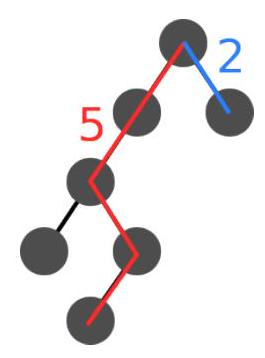
\includegraphics[width=3cm]{2022_11_23_3d3b162f8463b52386b8g-3}

In dem Beispiel oben hat der angegebene Binärbaum den kürzesten Pfad der Länge 2 und der längste Pfad sei dabei 5. In diesem Fall würde die Funktion 3 zurückgeben.

\begin{itemize}
  \item []\inputminted{Haskell}{A6_5.hs}
\end{itemize}

\end{document}